\documentclass[a4paper,12pt]{article}
\usepackage[english,vietnamese]{babel}
\usepackage{amsmath}
\usepackage{amssymb}
\usepackage{graphicx}
\usepackage{hyperref}
\usepackage{lmodern}
\usepackage{mathtools}
\usepackage{siunitx}

\newcommand{\exercise}[1]{\noindent\textbf{#1.}}
\newcommand{\sifrac}[2]{\displaystyle\SI[per-mode=fraction]{#1}{#2}}

\title{Numerical Methods: Heat Transfer}
\author{Nguyễn Gia Phong--BI9-184}
\date{\dateenglish\today}

\begin{document}
\maketitle

Given a bar of length $L = \SI{0.4}{\meter}$ consisting of homogeneous
and isotropic material with the initial temperature of $T_0 = \SI{0}{\celsius}$.
Suppose it is perfectly insulated with the exception of the ends with
the temperature of $T_g = \SI{100}{\celsius}$ and $T_d = \SI{50}{\celsius}$.
The thermal properties of material will be taken constant.
\begin{itemize}
  \item Specific heat capacity:
    $c_p = \sifrac{900}{\joule\per\kilogram\per\celsius}$
  \item Thermal conductivity:
    $\lambda = \sifrac{237}{\watt\per\meter\per\celsius}$
  \item Density:
    $\rho = \sifrac{2700}{\kilogram\per\cubic\meter}$
  \item Thermal diffusivity:
    $\alpha = \dfrac{\lambda}{\rho c_p}
            = \sifrac{9.753e-5}{\square\meter\per\second}$
\end{itemize}

The heat transfer in this bar can be described by the following
partial differential equation
\[\frac{\partial T}{\partial t}
  = \alpha\frac{\partial^2 T}{\partial x^2}\tag{$*$}\]
where the temperature $T$ is a function of postition $x$ and time $t$.

To solve the problem numerically, we devide space and time into equal intervals
of norms $\Delta x$ and $\Delta t$ respectively and let $M = L/\Delta x$.
Consequently, the spartial coordinate is defined as $x_i = (i - 1)\Delta x$
with $i \in [1\,..\,M + 1]$ and the temporal one is $t_n = n\Delta t$
with $n \in \mathbb N^*$. With these definitions\footnote{I believe $i = 0$
and $n = 0$ in the assignment papers are typos since then the domain of $x_i$
would exceed $L$ and $t_0$ would be negative.}, we denote $T_i^n = T(x_i, t_n)$.
Using numerical methods, we may start approximating the solutions of ($*$).

\begin{enumerate}
  \item The left-hand side of ($*$) can be approximated as
    \[\frac{\partial T}{\partial t} = \frac{T_i^{n+1} - T_i^n}{\Delta t}\]
  \item Similarly, the right-hand side is expressed in the following form
    \[\alpha\frac{\partial^2 T}{\partial x^2}
      = \alpha\frac{T_{i+1}^n - 2T_i^n + T_{i-1}^n}{\Delta x^2}\]
  \item ($*$) is therefore reformulated as
    \[\frac{T_i^{n+1} - T_i^n}{\Delta t}
      = \alpha\frac{T_{i+1}^n - 2T_i^n + T_{i-1}^n}{\Delta x^2}\]
  \item From the formular above
    and let $\beta = \alpha\dfrac{\Delta t}{\Delta x^2}$,
    we get
    \[T_i^{n+1} = T_i^n + \beta\left(T_{i+1}^n - 2T_i^n + T_{i-1}^n\right)\]
  \item Boundary conditions:
    \begin{itemize}
      \item $\forall n \in \mathbb N^*,\; T_1^n = T(0, t_n) = T_g$
      \item $\forall n \in \mathbb N^*,\; T_{M+1}^n = T(L, t_n) = T_d$
      \item $\forall i \in [2\,..\,M],\; T_{i}^1 = T(x_i, 0) = T_0$
    \end{itemize}
  \item From (4) and (5), the temperature at point $x_i$ of the bar
    at time $t_n$ is recursively defined as
    \[T_i^n = \begin{dcases}
        T_i^{n-1} + \beta\left(T_{i+1}^{n-1} - 2T_i^{n-1} + T_{i-1}^{n-1}\right)
        &\text{ if }1 < i \le M \land n > 1\\
        T_g &\text{ if }i = 1\\
        T_d &\text{ if }i = M + 1\\
        T_0 &\text{ otherwise}
      \end{dcases}\]
    Since the temperature only depends on the values in the past, values within
    $(i, n) \in [1\,..\,M+1]\times[1\,..\,N]$ with any $N$ of choice could
    be computed via dynamic programming:
    \begin{enumerate}
      \item Create a 2-dimensional dynamic array $T$ with one-based index
        and size $(M+1)\times 1$
      \item Initialize $T$ with $T_1^1 = T_g$, $T_{M+1}^1 = T_d$
        and $T_i^1 = T_0\ \forall i \in [2\,..\,M]$,
        where $T_i^n$ is element of row $i$ and column $n$
      \item For $n = 2$ to $N$
        \begin{itemize}
          \item Let $T_1^k = T_g$
          \item For $i = 2$ to $M$, let $T_i^k = T_i^{k-1}
            + \beta\left(T_{i+1}^{k-1} - 2T_i^{k-1} + T_{i-1}^{k-1}\right)$
          \item Let $T_{M+1}^k = T_d$
        \end{itemize}
      \item Return $T_i^n$
    \end{enumerate}
    Each iteration in (c) can be written in matrix notation as
    $T^k = AT^{k+1}$, where $T_n$ is column $n$ and $A$ is
    a matrix of size $(M+1)\times(M+1)$
    \[A =\begin{bmatrix}
        1 & 0 & 0 & \cdots & 0 & 0 & 0\\
        \beta & 1-2\beta & \beta & \cdots & 0 & 0 & 0\\
        0 & \beta & 1-2\beta & \cdots & 0 & 0 & 0\\
        \vdots & \vdots & \vdots & \ddots & \vdots & \vdots & \vdots\\
        0 & 0 & 0 & \cdots & 1-2\beta & \beta & 0\\
        0 & 0 & 0 & \cdots & \beta & 1-2\beta & \beta\\
        0 & 0 & 0 & \cdots & 0 & 0 & 1
      \end{bmatrix}\]
  \item Steps (a) to (c) is then implemented in Octave as
\begin{verbatim}
function T = heatrans (cp, lambda, rho, Tg, Td, T0, L,
                       dx, dt, N)
  alpha = lambda / rho / cp;
  beta = alpha * dt / dx^2;
  M = round (L / dx);
  side = repelem (beta, M);
  A = (diag (repelem (1 - 2*beta, M + 1))
       + diag (side, -1) + diag (side, 1));
  A(1, :) = A(end, :) = 0;
  A(1, 1) = A(end, end) = 1;

  T = repelem (T0, M + 1);
  [T(1) T(end)] = deal (Tg, Td);
  for k = 2 : N
    T(:, k) = A * T(:, k - 1);
  end
end
\end{verbatim}

    Choosing $\Delta x = \SI{0.01}{\meter}$, $\Delta t = \SI{0.5}{\second}$
    and $N = 841$, we define
\begin{verbatim}
T = heatrans (900, 237, 2700, 100, 50, 0, 0.4,
              0.01, 0.5, 841);
\end{verbatim}
    then the temperature at point $x_i$ at time $t_n$ is \verb|T(i, n)|.
    \pagebreak

    To visualize the heat transfer process, we use \verb|mesh| to plot
    a 3D graph:

    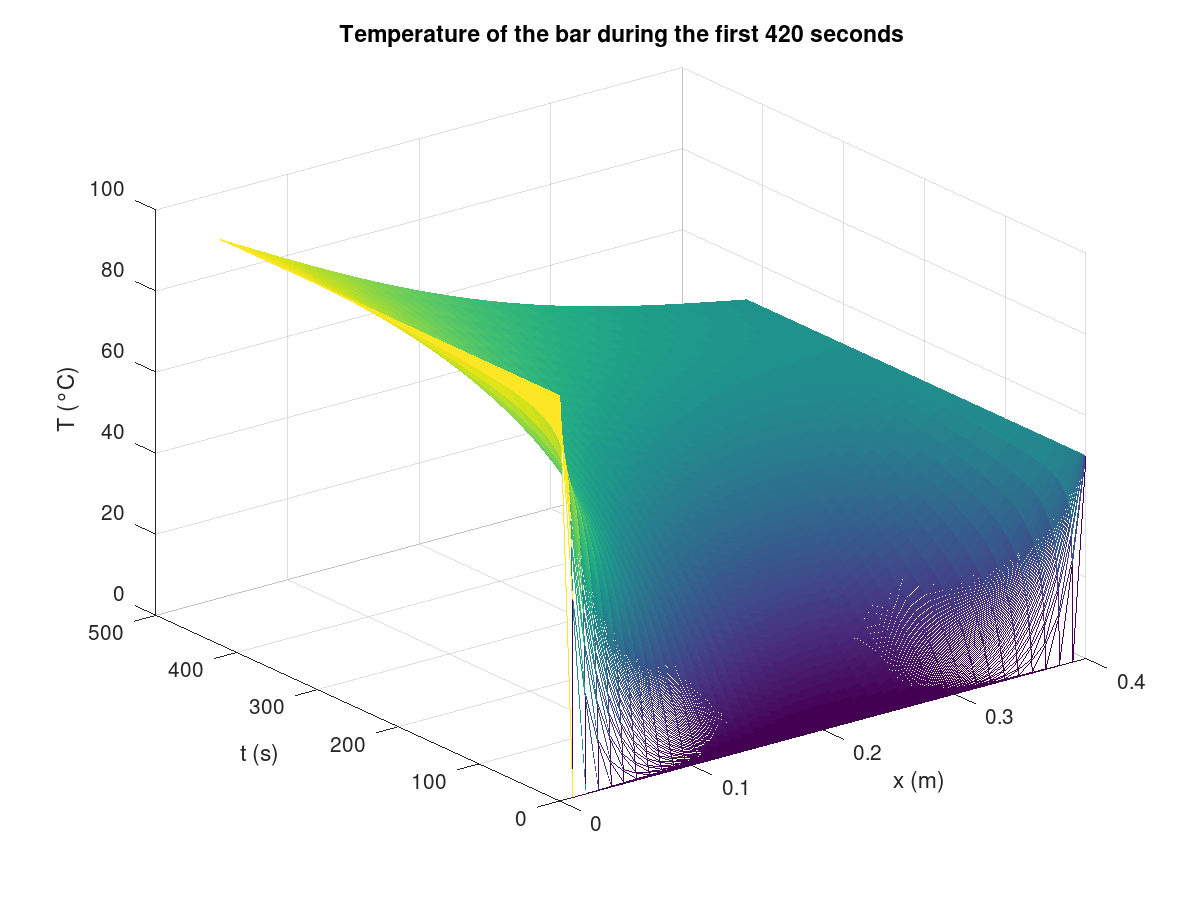
\includegraphics[width=0.841\textwidth]{mesh.png}

    The temperature can be shown more intuitively using \verb|contourf|:

    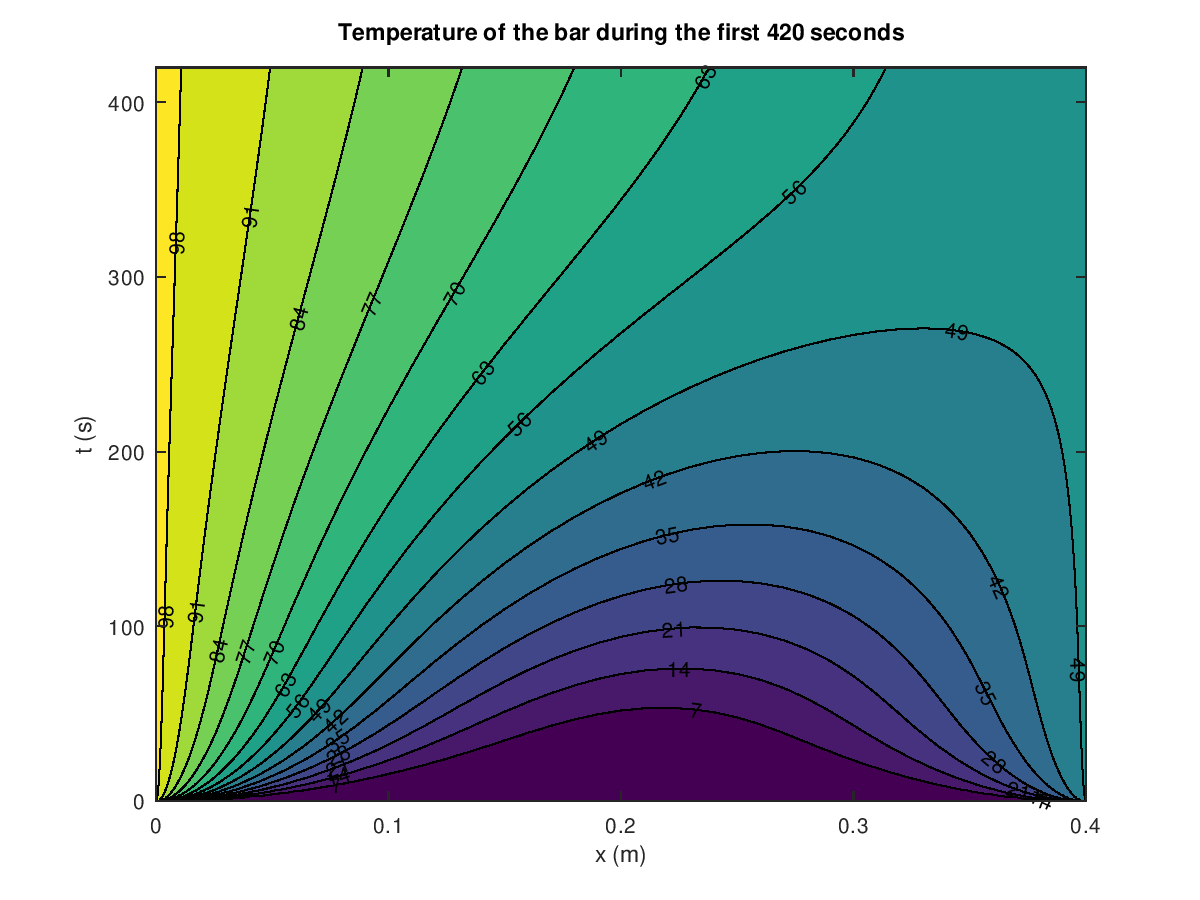
\includegraphics[width=0.841\textwidth]{contour.png}

    The \verb|script| to reproduce these results along with \verb|heatrans.m|
    bundled with this report and this document itself are all licensed under a
    \href{http://creativecommons.org/licenses/by-sa/4.0/}{Creative Commons
      Attribution-ShareAlike 4.0 International License}.
\end{enumerate}
\end{document}